\chapter{Machine Learning Fundamentals}
As machine learning techniques will be used for the classification of individual tap locations on a smartphone touchscreen, the following chapter will give a brief overview of the fundamental concepts evolving around statistical learning. Individual categories of learning algorithms will be discussed followed by two supervised-learning algorithms, namly Support Vector Machines and Neural Networks.

\section{Overview and Definition}

Ever since computers were invented, there has been a desire to enable them to learn \cite{samuel2000some}. This desire has grown into the field of machine learning which seeks to answer questions on how to build build systems that automatically improve with experience, and what the fundamental laws of learning processes are. Today, state-of-the-art ML covers a large set of methods and algorithms designed to accomplish tasks where conventional hard-coded routines have brought insufficient results. From speech recognition to email spam detection or recommendation systems, ML methods find broad usage in a variety of problem domains. \\

In order to understand what the principle of machine learning is, we will start with a definition by Samuel \cite{samuel2000some}:\\
\begin{quote}
\textit{Machine learning is the field of study that gives computers the ability to learn without being explicitly programmed.}\\
\end{quote}

In this definition, special emphasis is to be put on the last part of this definition. A computer is only then able to learn when he can perform a task without being explicitly instructed. Thus, in order to learn, the computer must somehow be able to instruct itself without the influence of an outer . As this definition lacks a more detailed view on what computer learning is, we will dive into a definition by Tom Mitchell \cite{mitchell2006discipline}:\\
\begin{quote}
\textit{A learning system is said to learn from experience E with respect to some class of tasks T and performance measure P, if its performance at tasks in T, as measured by P, improves with experience E.}\\
\end{quote}

The example that Mitchell notes, is one from the games of checkers \cite{mitchell2006discipline}. In this case checkers is the task T that the computer is aiming to learn. In order for the computer to learn, information on previously played matches is required. Since the computer does not know how to evaluate is a particular match was either good or bad, we set the performance to be defined based on how many matches were actually won. If a computer program can raise the amount of games won \textit{(performance measure P)} with the help of the experience from previously placed matches \textit{(experience E)} then it can learn to play checkers \textit{(task T)}. \\

% TODO: Maybe delete this.
To break this down into a more practical perspective, the challenge lies in finding an appropriate model in order to learn from data, which is the most common format to represent past experience. By learning, the computer adjusts parameters on the model based on the data that we feed the system with. Once the model has been adjusted, it can perform tasks with new incoming experience.

\section{Categorization of Methods}
As machine learning algorithms and methods differ from their approach to learning and underlying concepts, it is common practice to separate these into the following categories \cite{Duda:2000:PC:954544, Marsland:2009:MLA:1571643}  : Supervised learning, unsupervised learning, reinforcement learning and evolutionary learning. In the following sections I will briefly outline these.\\

\begin{itemize}

  \item[] \textbf{Supervised learning}, which is also named learning from example, is presumably the most prominent category of ML algorithms. The algorithm is given a training set of examples $\{x_0, \dots, x_n \}$, which are also known as \textit{features} and the correct target values $\{y_0, \dots, y_n \}$ mapped to each set of features, which is the answer that the algorithm should produce. The algorithm then generalizes based on the training set in order to respond with sensible outputs on all possible input values. Outputs, if they are discrete labels, correspond to a classification task whereas outputs on a continuous scale refer to a regression task (see \cite{Marsland:2009:MLA:1571643}).

An example for supervised learning is the classification of malignant or benign tumors as seen in cancer diagnosis. Let's assume we have a dataset with different properties of a tumor, such as the size or the color of the cells. These properties form our features $x$. Each set of features is mapped to an output label $y$ stating if the tumor is malignant or benign. The first step is to use the pairs $(x, y)$ of the training set to teach the algorithm the correct mapping of the problem space. As $x$ is linked to the output $y$ in the training set, learning the conjunction of these two values is done under supervision since the output label $y$ is given. Once learned, the algorithm is generalized to map unseen inputs to the correct output label.

Practical applications are for example digit and handwriting recognition \cite{lecun1990handwritten}, spam filtering \cite{guzella2009review} for e-mails or network anomaly detection \cite{lee2010uncovering}.

Presumably the most widely known machine learning techniques belong to this category, such as Support Vector Machines (SVMs), Artificial Neural Networks, Bayesian Statistics, Random Forests and Decision Trees \cite{Duda:2000:PC:954544}.\\

%TODO: add referation to how we will solve issues in the thesis.

  \item[] \textbf{Unsupervised learning} is the task of learning structures from input values that are not explicitly labeled. In comparison to supervised learning, where correct output values are provided for each input, unsupervised algorithms learn to identify similarities in the input data and can therefore group these \cite{Duda:2000:PC:954544}. These grouping problems are referred to as \textit{clustering}. The underlying idea here, is that humans learn by not explicitly being told what the right answer should be \cite{Marsland:2009:MLA:1571643}. If a human sees different species of snakes, for instance, he or she is able to identify them all as snakes. Hence, the human is aware that there are differences in each specific type of snake without specifically knowing a correct label.

A prominent example where unsupervised learning is heavily used, is in recommender systems for online retail shops. Amazon.com, for instance, uses a technique called \textit{collaborative filtering}, which measures similarity in customers based that they have previously bought \cite{linden2003amazon}. Having identified similar customers utilizing the cosine similarity, the algorithm can then recommend items that similar users have bought. This technique is also used for music recommendations \cite{perez2017recommender} or social network recommendations \cite{kautz1997referral}.

The field of unsupervised learning is closely related to density estimation in statistics, as with the density of inputs, we are able to group them. The K-means algorithm is the most prominent in this field \cite{Marsland:2009:MLA:1571643}.\\
  
  \item[] \textbf{Reinforcement learning} falls in between supervised and unsupervised learning methods. Whereas supervised learning tries to bridge the gap between input and corresponding output values and unsupervised methods detect groupings in incoming data, reinforcement learning is based on learning with a \textit{critic} \cite{Marsland:2009:MLA:1571643}. The algorithm tries different solution strategies to a problem and is told weather or not the answer provided was correct. An important fact here, is that the algorithm is not told how to correct itself. This practice of "trying-out" is based on the concept of \textit{trail-and-error learning} which is known as the \textit{Law-of-effect} \cite{Marsland:2009:MLA:1571643}. A good example is a child that tries to stand up and learn walking. The child tries out many different strategies for staying upright and receives feedback from the field based on how long it can stand without falling down again. The method that previously worked best is then repeated in order to find the optimal solution resulting in the child learning to walk \cite{Marsland:2009:MLA:1571643}.
  
 In more mathematical terms, the reinforcement learning problem is formalized with an agent and his environment. The environment in which the agent is set provides a set of \textit{states} on which the agent can perform \textit{actions} to maximize a certain \textit{reward}. By performing actions the state changes and a new reward is calculated. The reward then tells the agent if the action was a good choice. Goal of the algorithm is to maximize the reward \cite{Marsland:2009:MLA:1571643}.
 
 Reinforcement learning is a practical computational tool for constructing autonomous systems that improve themselves with experience. These applications have ranged from robotics, to industrial manufacturing, to combinatorial search problems such
as computer game playing \cite{kaelbling1996reinforcement}. 
Prominent methods of this category are Q-learning, Monte Carlo
methods and Hidden Markov Models \cite{Marsland:2009:MLA:1571643}.\\

  \item[] \textbf{Evolutionary learning} is inspired by strongly inspired by nature. As biological evolution improves the survival of a species, the strategy of adaptation to improve survival rates and the chance of offspring has inspired researchers to craft genetic algorithms (GA) \cite{Marsland:2009:MLA:1571643}. 

Genetic algorithms are a family of adaptive search procedures which have derived their name from the fact that they are based on models of genetic change in a population of individuals. These models have their foundation in three basic ideas: (1) Each evolutionary state of a population can be evaluated on a \textit{fitness} scale. This is done since biological evolution has a natural bias towards animals that are \" fitter \" than others. These animals tend to live longer, are more attractive and generate healthier and happier offspring, an idea which was originated in Charles Darwin's \"The Origin of Species\". (2) Each population can be mated to generate offspring using a \textit{mating operator}. (3) The third component are \textit{genetic operator}, such as \textit{crossover} and \textit{mutation}, which determine how the offspring solution is composed of the genetic material of the parents \cite{de1988learning}.

Evolutionary learning is often considered when other methods fail to find a reasonable answer. Algorithms find applications in search and mathematical optimization, but also in arts and simulation \cite{Marsland:2009:MLA:1571643}.\\
\end{itemize}

In this section we have seen several different problems that we can solved with the help of algorithmic learning. In this thesis, the focus is put on supervised learning as mapping the sensory data to the locations of tap event falls into this category. For predictions, two learning algorithms will be used which will be introduced in the following.

\section{Support Vector Machines}

A SVM is a non-linear kernel based extension of the so-called maximum margin classifier. Originating from binary classification problems, were $y \in \{1, -1\}$, the general idea of a maximum margin classifier is to find a separating hyperplane in the p-dimensional feature space. \\

This hyperplane separates the training examples leading to a maximum distance between the observations of the two classes \cite{James:2014:ISL:2517747}. This distance is referred to as margin $M$ measuring the smallest distance of a training observation towards the defined hyperplane. In order to find a suitable hyperplane only a subset of the training examples are sufficient.\\

Despite all that, linear separability is unlikely to be applicable to most real world problems. However, when a problem is linear separable, the constraint to the support vectors induce an undesirable sensitivity to individual observations, which can lead to high variance of the classifier. For this reason, the maximum margin classifier can be extended to it's more robust successor, the support vector classifier. Still being a linear classifier, the SVM allows for violations in fitting the margin. \\

Mathematically, the support vector classifier can be described via following optimization problem \cite{James:2014:ISL:2517747}:
\begin{eqnarray}
  & \max_{\beta, \epsilon} M \\
  & \textrm{subject to} \sum_{s=1}^{p} \beta^2_s = 1 \\
  g(x_{i}) &= y_i(\beta_0, \beta_1 x_1, \dots \beta_p x_p) \geq M(1 - \epsilon) \\
  & \epsilon \geq 0, \sum_{i=1}^n \epsilon_i \leq C
\end{eqnarray}

The objective of this optimization problem is to maximize the margin $M$ while choosing appropriate vector parameters $\beta$ and $\epsilon$. In this context, the parameter vector $\beta$ contains the coefficients of the hyperplane and the vector $\epsilon$ includes so-called slack variables that account for instances which are located on the wrong side of the margin and the hyperplane. These can be expressed as follows assuming that M is positive \cite{James:2014:ISL:2517747}:
\begin{equation}
  \epsilon_i =
  \begin{cases}
    0 & g(x_i) \geq M \\
    > 0 & M < g(x_i) < 0 \\
    > 1 & g(x_i) > 0 
  \end{cases}
\end{equation}

The hyperparameter C is a non-negative variable, which can be seen as a budget variable that allows for a certain sum of $\epsilon_i$ observations to be on the wrong side of the margin or hyperplane, respectively \cite{James:2014:ISL:2517747}. C manages the bias-variance tradeoff, since a low C tries to find a maximum margin hyperplane that almost exactly separates the two classes, resulting in low bias classifier for the available data set but in a high variance classifier for test data. Concurrently, allowing high budget C results in a high bias classifier that widens the margin, introducing more violations $\epsilon_i$ while reducing the variance of the classifier. Thereby C also controls the number of considered support vectors in dependence of the margin width.\\

Extending the support vector classifier to non-linear decision boundaries brings us to the SVM. Instead of extending the predictor space using higher order polynomials and interactions, SVM uses the so called ``kernel trick'' \cite{efron_hastie_2016}. In order to apply the ``kernel trick'' , i.a. \citeauthor{efron_hastie_2016} show that the optimization problem above can be rewritten as
\begin{equation}
  \^{f}(x) = \beta_0 + \sum_{i \in S} \alpha_i \langle x, x_i \rangle
\end{equation}

where $i \in S$ defines the subset of support vectors and $\langle x, x_i \rangle$ is the dot product of all pairs in the support vector. Thus, the parameters $\beta_0$ and $\sum_{i \in S}$ can be estimated with the help of least squares via simply computing the inner products of each pair in the support vector \cite{efron_hastie_2016}. The Expression in $\langle x, x_i \rangle$ can be generalized by a kernel function
\begin{equation}
  K(x_i,x_{i'}) = \sum_{s=1}^{p} x_{is} x_{i's}
\end{equation}
indicating the linear kernel that quantifies the distance between each pair in the data set \cite{James:2014:ISL:2517747}. Accordingly, the equation above can be rewritten as
\begin{equation}
  \^{f}(x) = \beta_0 + \sum_{i \in S} \alpha_i K(x, x_i)
\end{equation}
but in spite of restricting $K(\cdot, \cdot)$ to (3.7), we can now choose an arbitrary kernel function that maps our data into a high dimensional space where it is linearly separable. With this ``kernel trick'' the SVM can work in an implicitly enlarged predictor space, just by computing $\binom{n}{2}$  kernel functions $K(\cdot, \cdot)$, as opposed to an explicitly augmented predictor space, which is in fact computationally intractable \cite{James:2014:ISL:2517747}. In this work, we will be using a radial kernel function:
\begin{equation}
  K(x_i,x_{i'}) = \exp(-\gamma(\sum_{s=1}^{p}x_{is}x_{i's})^2),
\end{equation}
where $\gamma$ is a tuning parameter. After the parameters are learned on the basis of the training set, a new observation with the feature vector $x_0$ is classified via the following decision rule
\begin{equation}
  \^{f}(x) = sign(\beta_0 + \sum_{i \in S} \alpha_i K(x_i, x_{i'})).
\end{equation}
In view of the task at hand, an extension to multi-class classification of the SVM is utilized via one-versus-one classification. Given C classes, $\binom{C}{2}$ binary classifiers are learned in such a fashion that the C-th class is coded as $+1$ and the C0-th class as $1$. Consequently, a new instance is assigned to the class to which it was classified most frequently.
\newpage
\section{Neural Networks}
In this section, I will introduce neural networks which are interconnected systems used for supervised learning tasks. Besides the SVM, neural networks will be used in this thesis to predict the tap locations based on the collected motion data. Artificial neural networks are computing systems inspired by the biological neural networks found in animal brains. As these systems consist of several components, the first section will cover the neural units forming the fundamental processing unit of a network. After this, individual activation functions of these networks are discussed. In the last section the backpropagation algorithm which is used to train ANNs is explained.

\subsection{Neurons}

A neuron is fundamental processing unit of an artificial neural network. The diagram \label{fig:neuron} shows a model \cite{Haykin:1998:NNC:521706} of a neuron which consists of following components:
\begin{itemize}
  \item A set of \textit{connecting links} or \textit{synapses} which have a certain weight defined as the vector $\vec{w}$. The signal, represented as $\vec{x}$, flows through the \textit{synapse} and is mutipied by it's weight $w_i$.
  \item A \textit{adder} for summing the input signals and weights of the incoming synapses. These operations constitute a linear combiner.
  \item An \textit{activation function} $\varphi$ for limiting the amplitude of the output signal. This function is often referred to as the \textit{squashing function} since it squashing the possible output range \cite{Haykin:1998:NNC:521706}.
  \item An externally applied \textit{bias} $b$ which has the ability to lower or rise the net input to the activation function depending if the bias is negative or positive.
\end{itemize}
\begin{figure}[h]
	\centering
	\begin{tikzpicture}
    \node[draw,circle,minimum size=25pt,inner sep=0pt] (x) at (0,0) {$\Sigma$ $\varphi$};
    
      \node[inputNode] (x0) at (-3, 1.5) {$\tiny x_0$};
      \node[inputNode] (x1) at (-3, 0.75) {$\tiny x_1$};
      \node[inputNode] (x2) at (-3, 0) {$\tiny x_2$};
      \node[inputNode] (x3) at (-3, -0.75) {$\tiny x_3$};
      \node[inputNode] (xn) at (-3, -1.75) {$\tiny x_n$};

      \node[inputNode] (b) at (-0.12, 2) {$\tiny b_k$};
    
      \draw[stateTransition] (x0) to[out=0,in=120] node [midway, sloped, above=-2] {$w_{k0}$} (x);
      \draw[stateTransition] (x1) to[out=0,in=150] node [midway, sloped, above=-2] {$w_{k1}$} (x);
      \draw[stateTransition] (x2) to[out=0,in=180] node [midway, sloped, above=-2] {$w_{k2}$} (x);
      \draw[stateTransition] (x3) to[out=0,in=210] node [midway, sloped, above=-2] {$w_{k3}$} (x);
      \draw[stateTransition] (xn) to[out=0,in=240] node [midway, sloped, above=-2] {$w_{kn}$} (x);
      \draw[stateTransition] (x) -- (2,0) node [midway,above=-0.cm] {$\tiny h_k$};
      \draw[stateTransition] (b) -- (-0.12,0.44) node [midway, above=-0cm] {};
      \draw[dashed] (0,-0.43) -- (0,0.43);
      \node (dots) at (-3, -1.15) {$\vdots$};
  \end{tikzpicture}
  \caption{The diagram shows an artificial neuron's model with it's individual components.}\label{fig:neuron}
\end{figure}

Mathematically, a neuron $k$ can be expressed with the following equation \cite{Haykin:1998:NNC:521706}
\begin{eqnarray}
  u_k &= \sum_{j = 1}^{m}w_{kj}x_{j} \\
  h_k &= \varphi(u_k + b_k)
\end{eqnarray}
where $x_1, \dots, x_n$ are the input signals; $w_{k1}, \dots, w_{kn}$ refer to the synaptic weights of the neuron; $u_k$ is the linear combiner output of the summation on which the bias $b$ is added. The output of the neuron is expressed as $h_k$.

\subsection{Activation Functions}
The activation function $\varphi(u_k)$ denotes the output of the neuron $k$ and forms the junction between the neuron's input $x_k$ and output $h_k$. In order for the network to learn any complex non-linear function, each neuron in the networks requires a non-linear activation function \cite{Goodfellow-et-al-2016}. In this context, one commonly used function is the s-shaped \textit{sigmoid function} of which the \textit{logistic function} \cite{Haykin:1998:NNC:521706} is an example:\\

\begin{equation}
 \varphi(v) = \frac{1}{1 + \exp(-v)} 
\end{equation}
% \\
% However, as the logistic function outputs are in range $(0, 1)$,  A second popular function to consider is the \textit{hyperbolic tangent function}:\\

% \begin{equation}
%   \varphi(v) = \tanh(v)
% \end{equation}
% \\
The logic function, as in \ref{fig:af}, is well suited for classification as it is a non-linear function and it transforms the output values to either side of the curve. This results in a clear distinction between classes. However, the function has a compact domain range, meaning that the logistic function squashes output values into ranges $(0, 1)$. Consequently, when the inputs of a neuron become large, the function saturates at 0 or 1 with a derivative in these points being close to 0. As the derivatives are used for training the network\footnote{The training is performed via the backpropagation algorithm which is explained in section \ref{sec:backprop}}, the network trains slower if the weights or biases are high. This is referred to in literature as the \textit{vanishing gradient problem} \cite{Nair:2010:RLU:3104322.3104425}.\\

\begin{figure}[h!]
  \centering
  \begin{minipage}{.5\textwidth}
    \centering
    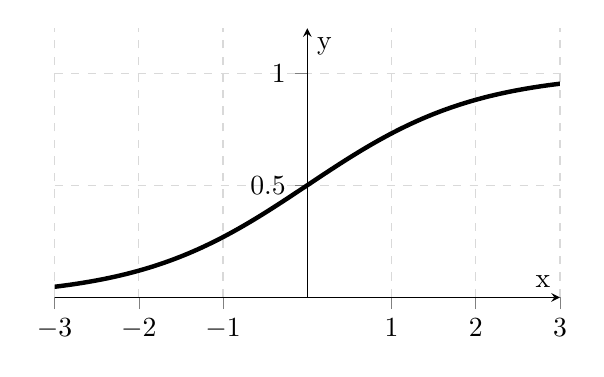
\begin{tikzpicture}
      \begin{axis}[
        legend pos=north west,
          axis x line=middle,
          axis y line=middle,
          width=8cm,
          height=5cm,       
          % x tick label style={/pgf/number format/fixed,
          %                     /pgf/number format/fixed zerofill,
          %                     /pgf/number format/precision=1},
          % y tick label style={/pgf/number format/fixed,
          %                     /pgf/number format/fixed zerofill,
          %                     /pgf/number format/precision=1},
          grid = major,
          grid style={dashed, gray!30},
          xmin=-3,
          xmax= 3,
          ymin= 0,
          ymax= 1.2,
          xlabel=x,
          ylabel=y,
          tick align=outside,
          enlargelimits=false]
        \addplot[black, ultra thick,samples=500] {1/(1 + exp(-x))};
      \end{axis}
    \end{tikzpicture}
    \label{fig:test1}
  \end{minipage}%
  \begin{minipage}{.5\textwidth}
    \centering
    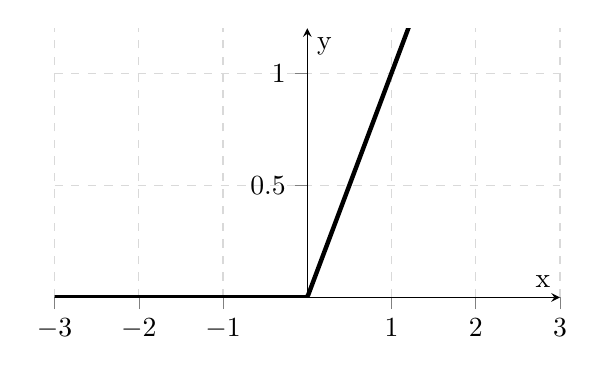
\begin{tikzpicture}
      \begin{axis}[
        legend pos=north west,
          axis x line=middle,
          axis y line=middle,
          width=8cm,
          height=5cm,
          % x tick label style={/pgf/number format/fixed,
          %                     /pgf/number format/fixed zerofill,
          %                     /pgf/number format/precision=1},
          % y tick label style={/pgf/number format/fixed,
          %                     /pgf/number format/fixed zerofill,
          %                     /pgf/number format/precision=1},
          grid = major,
          grid style={dashed, gray!30},
          xmin=-3,
          xmax= 3,
          ymin= 0,
          ymax= 1.2,
          xlabel=x,
          ylabel=y,
          tick align=outside,
          enlargelimits=false]
        \addplot[black, ultra thick,samples=500] {max(0, x))};
      \end{axis}
    \end{tikzpicture}
  \end{minipage}%
  \caption{The figure shows a plot of the hyperbolic  tangent  activation function on the left and a plot of the ReLU activation function on the right.}\label{fig:af}
\end{figure}


In order to avoid saturation problems, a commonly used non-linear activation function is the Rectified Linear Unit (ReLU) function \cite{Nair:2010:RLU:3104322.3104425}, which can be seen in figure \ref{fig:af}:\\

\begin{equation}
  \varphi(v) = \max(0, v)
\end{equation}
\\
ReLUs are non-saturating which results in a neuron always learning if the input is positive. Networks with ReLUs train several times faster and have become, as of 2015, the standard activation function for deep neural networks \cite{lecun2015deep}.

\subsection{Feedforward neural networks}
A feedforward neural network, or multilayer perceptron (MLP), is an ANN which consists of layers $L$ of neural units. The goal of a feedforward network is to approximate some function $f^*$ \cite{Goodfellow-et-al-2016}. In terms of a classifier, $y=f^*(x)$ maps an input $x$ to a label $y$. Consequently, a neural network with $m$ input nodes and 1 output node serves as a function with m inputs and 1 output.

\begin{figure}[h]
  \centering
  \def\layersep{3cm}
	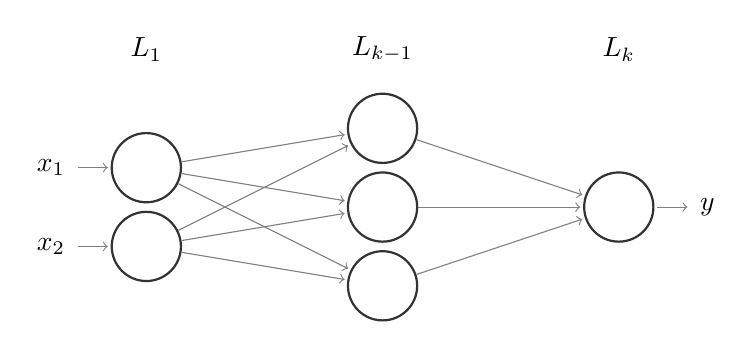
\begin{tikzpicture}[shorten >=1pt,->,draw=black!50, node distance=\layersep]
    \tikzstyle{every pin edge}=[<-,shorten <=1pt]
    \tikzstyle{neuron}=[circle,draw=black!80, thick,minimum size=25pt,inner sep=0pt]
    \tikzstyle{input neuron}=[neuron];
    \tikzstyle{output neuron}=[neuron];
    \tikzstyle{hidden neuron}=[neuron];
    \tikzstyle{annot} = [text width=4em, text centered]

    % Draw the input layer nodes
    \foreach \name / \y in {1,...,2}
    % This is the same as writing \foreach \name / \y in {1/1,2/2,3/3,4/4}
        \node[input neuron, pin=left:$x_{\y}$] (I-\name) at (0,-\y) {};

    % Draw the hidden layer nodes
    \foreach \name / \y in {1,...,3}
        \path[yshift=0.5cm]
            node[hidden neuron] (H-\name) at (\layersep,-\y cm) {};

    % Draw the output layer node
    \node[output neuron,pin={[pin edge={->}]right:$y$}, right of=H-2] (O) {};

    % Connect every node in the input layer with every node in the
    % hidden layer.
    \foreach \source in {1,...,2}
        \foreach \dest in {1,...,3}
            \path (I-\source) edge (H-\dest);

    % Connect every node in the hidden layer with the output layer
    \foreach \source in {1,...,3}
        \path (H-\source) edge (O);

    % Annotate the layers
    \node[annot,above of=H-1, node distance=1cm] (hl) {$L_{k-1}$};
    \node[annot,left of=hl] {$L_1$};
    \node[annot,right of=hl] {$L_k$};
\end{tikzpicture}
\caption{The diagram shows the structure of a typical feedforward network. The network has two input units in the input layer $L_1$ and one output unit in the output layer $L_k$. Layers $L_{2} \dots L_{k-1}$ the the so-called hidden layers.}\label{fig:ffnn}
\end{figure}
The network is named feedforward as it the information flowing through the network passes with the outermost input layer and and ends at the output unit of the output layer \cite{Goodfellow-et-al-2016}. All units in a layer are fully connected to the succeeding layer, however, there is no interconnection between units in the same layer. Figure \ref{fig:ffnn} shows a typical feedforward architecture with three layers including a single hidden layer $L_{k-1}$.\\

Considering equation (3.11) from the neuron section, we can now compute the input to the output node, given by\\
\begin{equation}
  \sum_{k=1}^{n} \alpha_k h_k
\end{equation}
\\
where $h_k$ is the output of the $k$th hidden node and $\alpha_k$ being the weight from the $k$th hidden to the output node. The output unit's activation function is then applied to this value, transforming the output to the given equation

\begin{equation}
  y = \varphi\left(\sum_{k=1}^{n} \alpha_k \varphi \left(\sum_{i=1}^{m} w_{ik} x_i + b \right)\right).
\end{equation}.

\subsection{Backpropagation}
\label{sec:backprop}
The purpose of the backpropagation algorithm \cite{rumelhart1988learning} is to adjust the synaptic weights of the network to approximate the function mapping between the inputs $x$ of the training data with the corresponding output labels $y$. The algorithm describes the process of training. The result of this algorithm is a neural network configured to minimize the error when solving a supervised learning task.\\

As a first step, the weights of the network are initialized which is usally done in a randomly manner or based on a certain heuristic. Then, each input pattern $p$, with features $p = \{x_0,x_1, x_2, \dots, x_n \}$ and label $y$, is then sequentially processed, layer by layer, by the network in two phases. In the first phase, the \textit{forward phase}, the ouput of the network is computed. The error function for the output nodes j are then calculated as follows, where $\hat{y}_j$ denotes the output node's generated output and $y_j$ is the desired ouput:

\begin{equation}
  E = \frac{1}{2}\sum_{j} (\hat{y}_j - y_j)^2.
\end{equation}

Continuing in the \textit{backward phase}, the network measures how much each neuron in the output layer $L_k$ has contributed to each output neuron's error. Furthermore, as to measure the error contributions coming from each neuron in the previous layer, this step is repeated until the input layer is reached and all error contributions, the gradients, are computed. To put this in other words, the \textit{backwards phase} measures the error gradients across all connection weights in the network by propagating the error gradients back into the network. \\

In this iterative process, the error gradients of the error function are calculated based on the partial derivative with respect to each connecting weight. If we define $o_j$ as output of a neural unit with
\begin{equation}
  o_j = \varphi(net_j)
\end{equation}
and the units input as 
\begin{equation}
  net_j = \sum_{j=1}^{n}x_{i}w_{ij},
\end{equation}
the chain rule can be applied in order to compute the partial derivatives as follows:
\begin{equation}
  \frac{\delta E}{\delta w_{ij}} = \frac{\delta E}{\delta o_j} \frac{\delta o_j}{\delta net_j} \frac{\delta net_j}{\delta w_{ij}}
\end{equation}

Given the partial derivative in respect to the weight $w_{ij}$, the change of the weight $\Delta w_{ij}$ can be determined. Here, the weight update equation (3.22) is computed depending on two cases. Either if the node $j$ is in the hidden layer or in the output layer:
\begin{equation}
  \Delta w_{ij} = -\eta \frac{\delta E}{\delta w_{ij}} = - \eta \delta_j o_i
\end{equation}

\begin{equation}
  \delta_j =
  \begin{cases}
    \varphi'(net_j)(o_j - \hat{y}_j) & \text{node $j \in L_k$}\\
    \varphi'(net_j) \sum_k \delta_k w_{jk} & \text{node $j \notin L_k$}
  \end{cases}
\end{equation}
\\
In equation (3.23), $\eta$ denotes the \textit{learning rate}, which defines to which amount the reverse gradients are applied to the weight update; $k$ refers to a node in the successor layer of the node $j$.\\

Once the weights are updated, the global error of the network is calculated and the forward and the backward phase are repeated for the rest of the training patterns. One pass through all of the training patterns is called a \textit{training
epoch}. Several strategies exist to stopping the described training process. One condition is to stop after to a fixed number of training epoches, a second can be a stop once the change in the weights reaches a certain low-end threshhold. After the process, the final values of the weights are saved and can be used for prediting new incoming patterns.

% \subsection{Recurrent Neural Networks}
% In the previous section, we have looked at feedforward neural networks where information, as the name implies, flows only in one direction, from the input layer to the output layer. A recurrent neural network (RNN) is similar to a feedforward network, except that it also has cyclic connections. This structure makes a RNN able to memorize previous information that has flown throw the network.\\

% For each timestep $t$, the recurrent neuron, as illustrated in Figure bla, recieves the input $x_{(t)}$ as well as it's own ouput from the the previously compututed time step $y_{(t_{-1})}$. The network can then be transformed to represent the time axis, as illustrated in Figure bla, which is also refered to as \textit{unrolling through time}.\\

% In comparison to the feedforward neuron, the recurrent neuron has a pair of wights: one represents the inputs $x_{(t)}$ and the other for the ouput of the previous step $y_{(t_{-1})}$. We can define these weight vectors as $w_x$ and $w_y$. The output of a recurrent neuron can then be computed with following equation:\\

% \begin{equation}
% y(t) = \varphi \left( x_{(t)}^T  w_{x} + y_{t-1}^T  w_y + b \right)
% \end{equation}
% \\
% where $b$ refers to the \textit{bias} of the node.

% \subsection{Long-short term memory}
% As the RNN gains it's possibility to remember because of the recurrent neuron \textit{recurrent connection}, in practise, RNNs can forget patterns after a small amount of steps. Therefore, it is hard to train a RNN to identifiy time correlations of longer sequences. As we will be analyzing the time series data produced from the sensor components of the smartphone, I would like to introduce a varient of the RNN, called Long Short-Term Memory (LSTM).

% \begin{figure}
%   \centering
%   \begin{tikzpicture}[
%     prod/.style={circle, draw, inner sep=0pt},
%     ct/.style={circle, draw, inner sep=5pt, ultra thick, minimum width=10mm},
%     ft/.style={circle, draw, minimum width=8mm, inner sep=1pt},
%     filter/.style={circle, draw, minimum width=7mm, inner sep=3pt},
%     mylabel/.style={font=\scriptsize\sffamily},
%     >=LaTeX
%     ]

% \node[ct, label={[mylabel]Cell}] (ct) {$c_t$};
% \node[filter, right=of ct] (int1) {$\varphi$};
% \node[prod, right=of int1] (x1) {$\times$}; 
% \node[right=of x1] (ht) {$h_t$};
% \node[prod, left=of ct] (x2) {$\times$}; 
% \node[filter, left=of x2] (int2) {$\varphi$};
% \node[prod, below=5mm of ct] (x3) {$\times$}; 
% \node[ft, below=5mm of x3, label={[mylabel]right:Forget Gate}] (ft) {$f_t$};
% \node[ft, above=of x2, label={[mylabel]left:Input Gate}] (it) {$i_t$};
% \node[ft, above=of x1, label={[mylabel]left:Output Gate}] (ot) {$o_t$};

% \foreach \i/\j in {int2/x2, x2/ct, ct/int1, int1/x1,
%             x1/ht, it/x2, ct/it, ct/ot, ot/x1, ft/x3}
%     \draw[->] (\i)--(\j);

% \draw[->] (ct) to[bend right=45] (ft);

% \draw[->] (ct) to[bend right=30] (x3);
% \draw[->] (x3) to[bend right=30] (ct);

% \node[fit=(int2) (it) (ot) (ft), draw, inner sep=0pt] (fit) {};

% \draw[<-] (fit.west|-int2) coordinate (aux)--++(180:7mm) node[left]{$x_t$};
% \draw[<-] ([yshift=1mm]aux)--++(135:7mm);
% \draw[<-] ([yshift=-1mm]aux)--++(-135:7mm);

% \draw[<-] (fit.north-|it) coordinate (aux)--++(90:7mm) node[above]{$x_t$};
% \draw[<-] ([xshift=1mm]aux)--++(45:7mm);
% \draw[<-] ([xshift=-1mm]aux)--++(135:7mm);

% \draw[<-] (fit.north-|ot) coordinate (aux)--++(90:7mm) node[above]{$x_t$};
% \draw[<-] ([xshift=1mm]aux)--++(45:7mm);
% \draw[<-] ([xshift=-1mm]aux)--++(135:7mm);

% \draw[<-] (fit.south-|ft) coordinate (aux)--++(-90:7mm) node[below]{$x_t$};
% \draw[<-] ([xshift=1mm]aux)--++(-45:7mm);
% \draw[<-] ([xshift=-1mm]aux)--++(-135:7mm);
% \end{tikzpicture}
% \caption{The figure shows a LSTM cell.}
% \end{figure}
